\documentclass[a4paper]{scrreprt}
	
\usepackage[T1]{fontenc}
\usepackage[ngerman]{babel}     % deutsche Silbentrennung
\usepackage[utf8x]{inputenc}    % wegen deutschen Umlauten & UTF-8
\usepackage{lmodern}		% Schönere Schriftart
\usepackage{graphicx}           % Grafikpaket laden
\usepackage{amsmath,amssymb}    % Mathe
\usepackage{tikz}               % Zeichungen
\usepackage{hyperref}		% Links
\hypersetup{			% Link-Formatierung entfernen & pdf-Inforamtionen setzten
	pdfauthor={Maximilian Awiszus, Holger Ebhart, Lidia Grigoriev, Paul Jungeblut, Philipp Kern  und Matthias Schimek},
	pdftitle={Visualizing Trends. Was verrät uns Twitter?},
	colorlinks,
	citecolor=black,
	filecolor=black,
	linkcolor=black,
	urlcolor=black
}
\usepackage{microtype}		% font expansion
\usepackage{enumerate}

\title{Praxis der Softwareentwicklung:\\Visualizing Trends. Was verrät uns Twitter?}
\subtitle{Pflichtenheft}
\author{Maximilian Awiszus\and Holger Ebhart\and Lidia Grigoriev\and Paul Jungeblut\and Philipp Kern\and Matthias Schimek}
\date{
\includegraphics[width=.3\textwidth]{img/logo.pdf}\\\vspace{3mm}WS 2014/15}

\begin{document}
	\maketitle
	\setcounter{tocdepth}{1}
	\tableofcontents

	\chapter{Einführung}
		% vollständige Beschreibung der Aufgabenstellung.
	
	\chapter{Datenbank}
	\label{chap:datenbank}
		\section{Datenbankzugriff}\label{sec:datenbankzugriff}
Die zentrale Komponente unseres Systems ist die Datenbank. In sie fügt der Crawler neue Datensätze ein und aktualisiert Vorhandene. Der Kategorisierer ist dafür zuständig die gefundenen Accounts nach der DMOZ.org Datenbank in Kategorien zu unterteilen. Die GUI wiederum ist die Komponente die die Daten aus der Datenbank ausliest und visualisiert. Gegebenenfalls kann sie auch Einträge hinzufügen, verändern beziehungsweise vervollständigen.
\\Da alle unsere drei Systemkomponenten lesend, sowie schreibend auf die Datenbank zugreifen, haben wir uns entschlossen ein Paket für den Datenbankzugriff für alle Komponenten zur Verfügung stellen. Dieses sogenannte mysql-Package ist dann für den Auf- und Abbau der Verbindung zur Datenbank zuständig, sowie für das Schreiben und Lesen in beziehungsweise aus der Datenbank. Es stellt für jede der drei Komponenten ein eigenes Interface zur Verfügung, sodass jede Komponente nur die für sie erlaubten Änderungen an der Datenbank vornehmen kann.
In \cref{fig:mysql-package} ist der Aufbau des mysql-Packages zu sehen. Das darin eingeschlossene result-Package stellt Objekt und Methoden zu Verfügung um die Ergebnisse aus der Datenbank zu speichern und zu verarbeiten.

\begin{figure}[h!]
	\centering
	\includegraphics[width=\textwidth,height=\textheight,keepaspectratio=true]{dia/uml_mysql-package}
	\caption{UML-Klassendiagramm des mysql-Packages}
	\label{fig:mysql-package}
\end{figure}

\begin{description}
	\item[AccessData] Klasse zur Verwaltung von Zugriffsdaten für die Datenbank.
	\item[DBConnection] Abstrakte Klasse die eine Verbindung zu einer Datenbank aufbaut und diese Verbindung auch wieder trennt.
	\item[DBIcrawler] Interface, welches die Methoden spezifizieren die der Crawler für den Datenbankzugriff benötigt.
	\item[DBIcategorizer] Interface, welches die Methoden spezifizieren die der Kategorisierer für den Datenbankzugriff benötigt.
	\item[DBIgui] Interface, welches die Methoden spezifizieren die die GUI für den Datenbankzugriff benötigt.
	\item[DBcrawler] Diese Klasse implementiert die Methoden des DBIcrawler Interfaces und stellt dem Crawler eine Datenbankverbindung zur Verfügung.
	\item[DBcategorizer] Diese Klasse implementiert die Methoden des DBIcategorizer Interfaces und stellt dem Kategorisierer eine Datenbankverbindung zur Verfügung.
	\item[DBgui] Diese Klasse implementiert die Methoden des DBIgui Interfaces und stellt dem der GUI eine Datenbankverbindung zur Verfügung.
	\item[Index] Als abstrakte Klasse stellt Index eine Möglichkeit zum Speichern des Datenbankindexes von Datenbankeinträgen zur Verfügung.
	\item[Account] In dieser Klasse werden einzelne Accounts verwaltet und gespeichert.
	\item[Retweets] In dieser Klasse werden nach Orten (und eventuell nach Daten) gruppierte Retweets verwaltet und gespeichert.
	\item[Tweets] In dieser Klasse werden nach Daten gruppierte Tweets verwaltet und gespeichert.
	\item[Location] In dieser Klasse werden einzelne Orte verwaltet und gespeichert.
	\item[Category] In dieser Klasse werden einzelne Kategorien verwaltet und gespeichert.
	\item[TweetsAndRetweets] Diese Klasse wird benutzt um zusammengefasste Daten der Datenbank an die GUI weiter zu leiten.
\end{description}

\section{ER-Modell}
Die Datenbank besteht aus sieben Tabellen, die über Fremdschlüssel miteinander in Relation stehen (s. \cref{fig:mysql-er}).
\begin{description}
	\item[accounts] Enthält alle verifizierten Accounts, die der Crawler im Twitter Stream mitgelesen hat, bzw. auch nicht verifizierte Accounts, die in der GUI hinzugefügt wurden. Dabei entspricht \emph{TwitterAccountId} der ID des Accounts in Twitter und \emph{id} ist ein Datenbank interner Primärschlüssel. Die Attribute \emph{Verified}, \emph{URL} und \emph{AccountName} entsprechen jeweils in Twitter hinterlegten Daten. \emph{Categorized} gibt an ob dieser Account bereits kategorisiert wurde und \emph{LocationId} Enthält den vom Loakaliserer berechneten zugehörigen Ort.
	\item[category] speichert die hierarchisch strukturierten (\emph{ParentId}) Kategorien.
	\item[accountCategory] Stellt die Relation zwischen	\emph{accounts} und \emph{category} in einer separaten Tabelle her, da einem Account mehrere Kategorien zugeordnet werden können.
	\item[location] Enthält die vom Lokalisierer ermittelten Orte, die jeweils \emph{Code} und \emph{Name} enthalten und auch per \emph{ParentId} hierarchisch gegliedert sein können.	
	\item[day] Enthält unterschiedliche Daten (\emph{Day}), die mittels \emph{Id} referenziert werden.
	\item[tweets] Beinhaltet die Anzahl der Tweets (\emph{Counter}) eines Accounts (\emph{AccountId}) an einem bestimmten Tag (\emph{DayId}).
	\item[retweets] Speichert die Anzahl der Retweets (\emph{Counter}) auf Tweets eines Accounts (\emph{AccountId}) an einem bestimmten Tag (\emph{DayID}) innerhalb eines bestimmten Lands bzw. Orts (\emph{LocationId}).
\end{description}
\begin{figure}[h!]
	\centering
	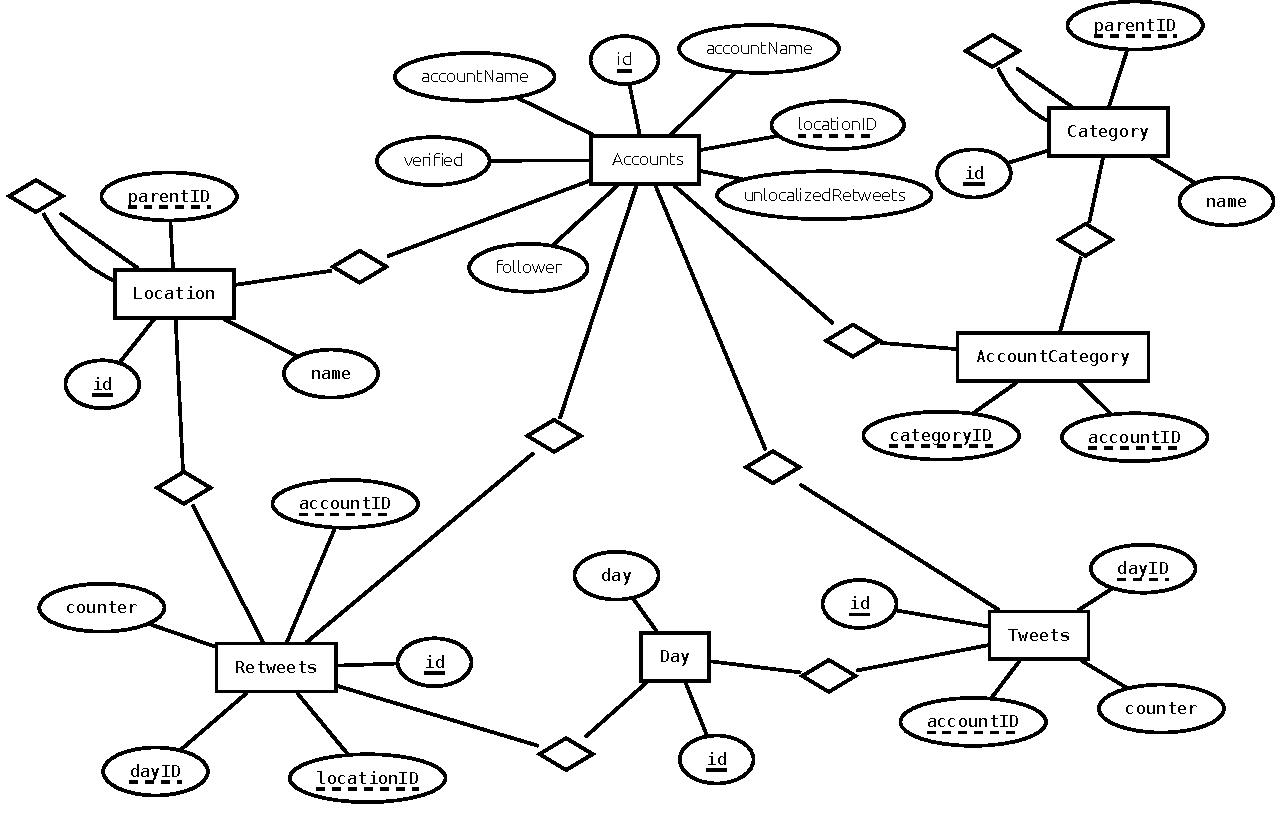
\includegraphics[width=\textwidth,height=\textheight, keepaspectratio=true]{dia/er}
	\caption{ER-Modell der MySQL-Datenbank}
	\label{fig:mysql-er}
\end{figure}

\section{Datenbankzugriff der GUI}
Da die GUI zur Visualisierung der Daten aus der Datenbank dient, ist es nötig, dass sie diese Daten in möglichst kompakter und vollständiger Form abrufen kann. Dazu stehen der GUI mehrere Möglichkeiten zur Verfügung die im Folgenden aufgelistet sind. Dabei sollen zum einen die Fähigkeiten der Datenbank ausgenutzt werden um Daten zusammenzufassen, zum Anderen sollen aber auch alle relevanten Daten einzeln zur Verfügung stehen.
\begin{description}
\item[Kategorien und Orte] Diese Informationen können jeweils als komplette Tabelle von der Datenbank geholt werden.
\item[Accounts] Mithilfe eines Account-Namens ist es möglich die AccountId herauszufinden. Außerdem kann mittels eines Worts nach Accounts gesucht werden, welche dieses Wort im Namen beinhalten.
\item[Tweets und Retweets] Um zu vorgegebenen Kategorien und Orten die Daten zu bekommen, sollen 4 Methoden zur Verfügung stehen. Im Folgenden werden jeweils nur die Tweets und Retweets von Accounts betrachtet, auf welche die Kategorie-Ort-Kombination/en passen.

\begin{itemize}
	\item Methoden welche über alle Kalenderdaten summieren:
	\begin{itemize}
		\item Eine Methode liefert jeweils die Summe der Tweets und Retweets pro Ort zurück, also für jeden Ort aus der Datenbank eine Summe von Tweets und eine Summe von Retweets.
		\item Eine weitere Methode liefert alle Accounts mit der Summe ihrer Tweets zurück auf die die Kategorie-Orts-Kombination passt. Dabei wird zu jeder Account-Orts Kombination eine Summe der Retweets mitgeliefert.
	\end{itemize}
	\item Methoden welche die Daten nach Kalenderdaten separieren:
	\begin{itemize}
		\item Eine Methode liefert für jede Ort-Datums Kombination, die Summe über alle Tweets und Retweets zurück, sodass dann zu jedem Ort zu jedem Datum eine Summe von Tweets und Retweets bekannt ist.
		\item Eine weitere Methode liefert alle betroffenen Accounts zurück und pro Account noch die Anzahl der Retweets pro Ort pro Tag und die Tweets pro Tag.
	\end{itemize}
\end{itemize}
Die Berechnungen werden so weit möglich in die Datenbank ausgelagert, sodass diese die Summation übernimmt. Dadurch kann die Geschwindigkeit der Datenbank ausgenutzt werden und die Ressourcen auf Client-Seite werden geschont.


\end{description}
	\chapter{Crawler}
	\label{chap:crawler}
		\section{Aufbau}

\subsection{Paketdiagramm}
In \cref{fig:crawler_package} ist die Grobstruktur des Crawlers als Paketdiagramm zu sehen.
\begin{figure}[h!]
	\centering
	\includegraphics[width=\textwidth,height=\textheight,keepaspectratio=true]{dia/crawler_package}
	\caption{Paketdiagramm des Crawlers}
	\label{fig:crawler_package}
\end{figure}

\begin{description}
\item[main] Dieses Paket beinhaltet die wesentliche Programmlogik.
\item[mysql] In diesem Paket sind Klassen, welche Methoden bereitstellen um auf eine MySQL-Datenbank zuzugreifen. Außerdem ist noch ein Paket mit Klassen zur Verwaltung von Twitter-Daten integriert.
\item[locate] Das locate-Paket dient zur Lokalisierung von Twitter-Accounts und Retweets mittels Webdiensten.
\item[java 1.8] Standard java 1.8 Bibliothek.
\item[twitter4j] twitter4j Bibliothek.
\end{description}

\subsection{Klassendiagramm}
Zum Sammeln von Daten von Twitter verwenden wir einen Crawler, welcher über die Twitter-API Daten sammelt. Dazu ist es nötig diese Daten zu empfangen, dann zu puffern und schlussendlich in die Datenbank zu schreiben. Allerdings müssen die Daten noch gefiltert werden, da wir nur Daten von verifizierten Twitter-Accounts (und manuell hinzugefügten) speichern. Sind die Daten gefiltert, werden sie vom Crawler noch lokalisiert. Das heißt, dass jedem Account beziehungsweise jedem Retweet eine Geoposition/Land zugeordnet wird. Ist dies erfolgt so werden die Daten in die Datenbank geschrieben.
\\ In \cref{fig:uml_crawler} ist der Aufbau des Crawlers anhand eines UML-Klassendiagramms spezifiziert.

\begin{figure}[h!]
	\centering
	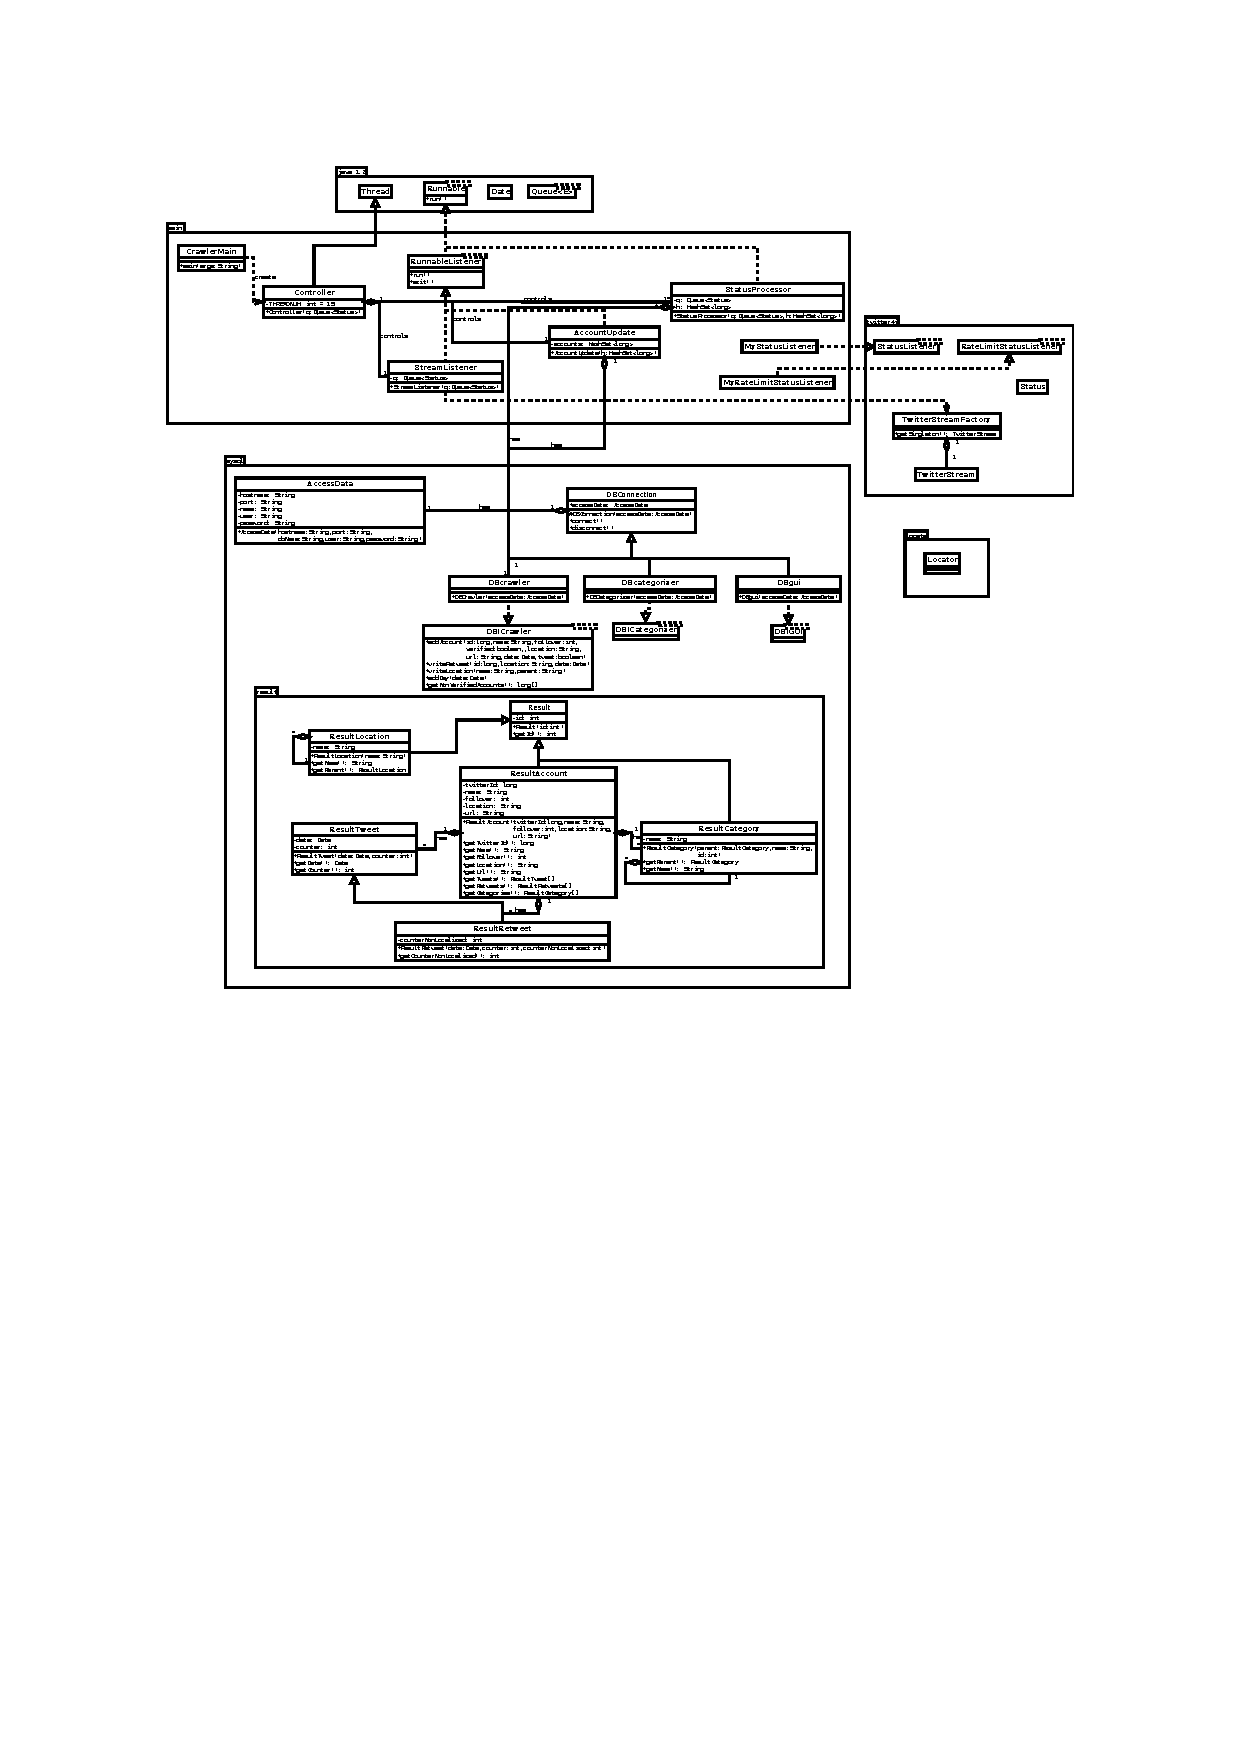
\includegraphics[width=\textheight,height=\textwidth,keepaspectratio=true,angle=-90]{dia/uml_crawler}
	\caption{UML-Klassendiagramm des Crawlers}
	\label{fig:uml_crawler}
\end{figure}

\begin{description}
\item[CrawlerMain] Klasse enthält die main-Methode zum Aufrufen des Programms. Sie überprüft die Eingabe für die Datenbankverbindung und startet einen Controller. Danach seht sie dem Benutzer über die Konsole zur Verfügung um das Programm zu überwachen.
\item[RunnableListener] Interface welches Runnable erweitert und zusätzlich noch eine exit-Methode fordert um Threads zu beenden.
\item[Controller] Diese Klasse koordiniert alle Aktionen die nötig sind um Daten bei Twitter abzuholen und in die Datenbank zu schreiben. Dazu startet sie einen StreamListener, ein AccountUpdate und mehrere StatusProcessors jeweils als Thread. Außerdem kontrolliert sie den Puffer und sorgt für ein sauberes Beenden des Programms indem alle Verbindungen ordnungsgemäß geschlossen und die Threads beendet werden.
\item[StreamListener] Stellt eine Verbindung zur Twitter-Streaming-API her und initialisiert einen MyStatusListener.
\item[AccountUpdate] Diese Klasse stellt eine Methode zur Verfügung um in der Datenbank periodisch nach Accounts zu suchen, welche manuell hinzugefügt wurden, nicht verifiziert sind, aber auch getracked werden sollen.
\item[StatusProcessor] Diese Klasse stellt die Funktionalität zur Filterung der Daten von Twitter zur Verfügung, welche sie aus dem Puffer nimmt. Außerdem bietet sie die Möglichkeit diese Daten in die Datenbank zu schreiben.
\item[MyStatusListener] Diese Klasse nimmt die Daten von Twitter entgegen und schreibt diese in einen Puffer.
\item[MyRateLimitStatusListener] Diese Klasse nimmt Meldungen von Twitter bezüglich RateLimits entgegen.
\item[Locator] Der Locator lokalisiert Accounts und Retweets mithilfe eines Webdienstes.
\end{description}

\section{Start des Crawlers}
Beim Starten des Crawlers werden sämtliche notwendigen Komponenten der Reihe nach gestartet. Dadurch wird garantiert, dass jede Komponente eine Umgebung vorfindet in der sie laufen kann und alle Ressourcen bereits zur Verfügung stehen. In \cref{fig:crawler_start} ist der Start des Crawlers beispielhaft mit 2 StatusProcessors dargestellt.

\begin{figure}[h!]
	\centering
	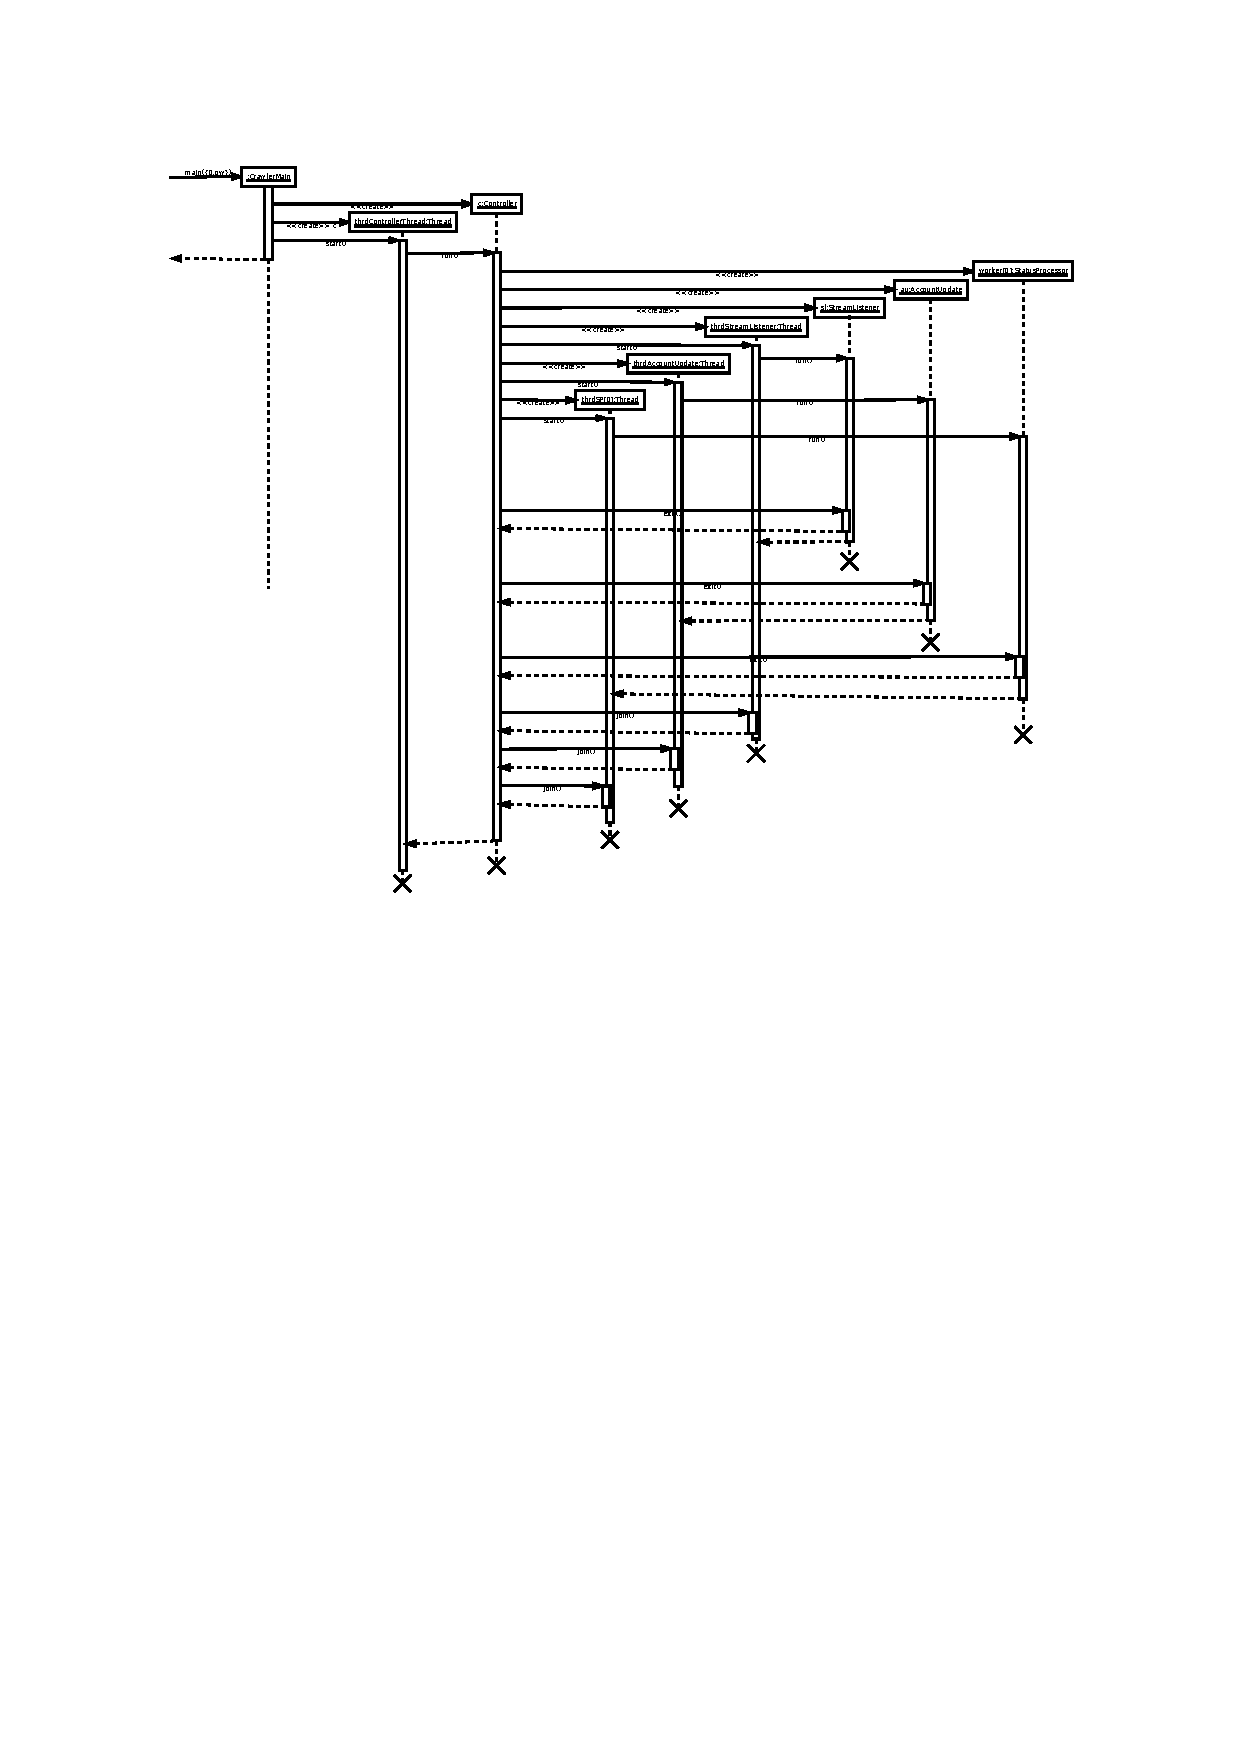
\includegraphics[width=\textheight,height=\textwidth,keepaspectratio=true,angle=-90]{dia/crawler_start_sequence}
	\caption{Sequenzdiagramm zum Start des Crawlers}
	\label{fig:crawler_start}
\end{figure}

Um den Crawler zu starten, werden ihm die Zugriffsdaten auf die Datenbank übergeben und die Anzahl der Threads die später Daten verarbeiten (Hardware abhängig).
Die main-Methode der Main-Klasse instantiiert daraufhin ein Controller Objekt, welches ab dann sämtliche Steuerung übernimmt. Diese Controller Objekt wird dann in einem Thread ausgeführt. Die Main-Klasse ist nun nur noch dafür zuständig Benutzereingaben entgegenzunehmen und diese weiter zu delegieren.
Sobald der Controller gestartet wurde instantiiert er die StatusProcessor Objekte, welche später sämtliche Daten verarbeiten müssen (deren Anzahl vom Benutzer festgelegt wird). Außerdem werden noch ein AccountUpdate- und ein StreamListener-Objekt instantiiert. Ersteres dient dazu eine Liste nicht verifizierter Accounts, die dennoch getracked werden sollen, aus der Datenbank aktuell zu halten. Zweiteres ist dafür zuständig eine Verbindung zur TwitterStream-API einzurichten. Alle diese Objekte werden dann vom Controller als eigenständige Threads ausgeführt.
Daraufhin beginnt der StreamListener eine Verbindung zur TwitterStreaming-API herzustellen (siehe \cref{fig:initialize_stream}).\\
Nun ist der Crawler im aktiven Zustand und empfängt Daten von Twitter, welche dann gefiltert, vervollständigt und in der Datenbank abgelegt werden.\\
Wird der Crawler vom Benutzer beendet, so sendet der Controller jedem Objekt, welches in einem Thread läuft ein exit-Signal. Daraufhin beenden die Objekte ihre Tätigkeit und der jeweilige Thread kehrt zum Controller zurück, sodass dieser dann das gesamte Programm beenden kann.
\\

\begin{figure}[h!]
	\centering
	\includegraphics[width=\textheight,height=\textwidth,keepaspectratio=true,angle=-90]{dia/crawler_initialize_stream}
	\caption{Sequenzdiagramm zur Initialisierung des TwitterStreams}
	\label{fig:initialize_stream}
\end{figure}

Um eine Verbindung zur Twitter-Streaming-API herzustellen, wird zuerst ein RateLimitStatusListener erstellt um auf Rate-Limits von Twitter zu reagieren. Danach wird noch ein Filter erstellt mit dem der Twitterstream durchsucht wird und ein MyStatusListener um über eingehende Daten benachrichtigt zu werden.
Anschließend wird ein TwitterStream-Objekt aus der twitter4j-Bibliothek geholt(ist Singleton). Auf diesem werden dann die Methoden zur Initialisierung aufgerufen und somit die Listener und der Filter gesetzt.\\
Zum Schließen des Streams wird auf dem TwitterStrem-Objekt die shutdown-Methode aufgerufen.

\section{Verarbeitung der Daten von Twitter}
Um zu verdeutlichen wie die Daten von Twitter innerhalb des Crawlers verarbeitet werden, ist in \cref{fig:crawler_process} der Datenfluss durch den Crawler exemplarisch dargestellt. Dabei werden die Daten von Twitter abgeholt, gepuffert, dann gefiltert und schlussendlich in die Datenbank geschrieben.

\begin{figure}[h!]
	\centering
	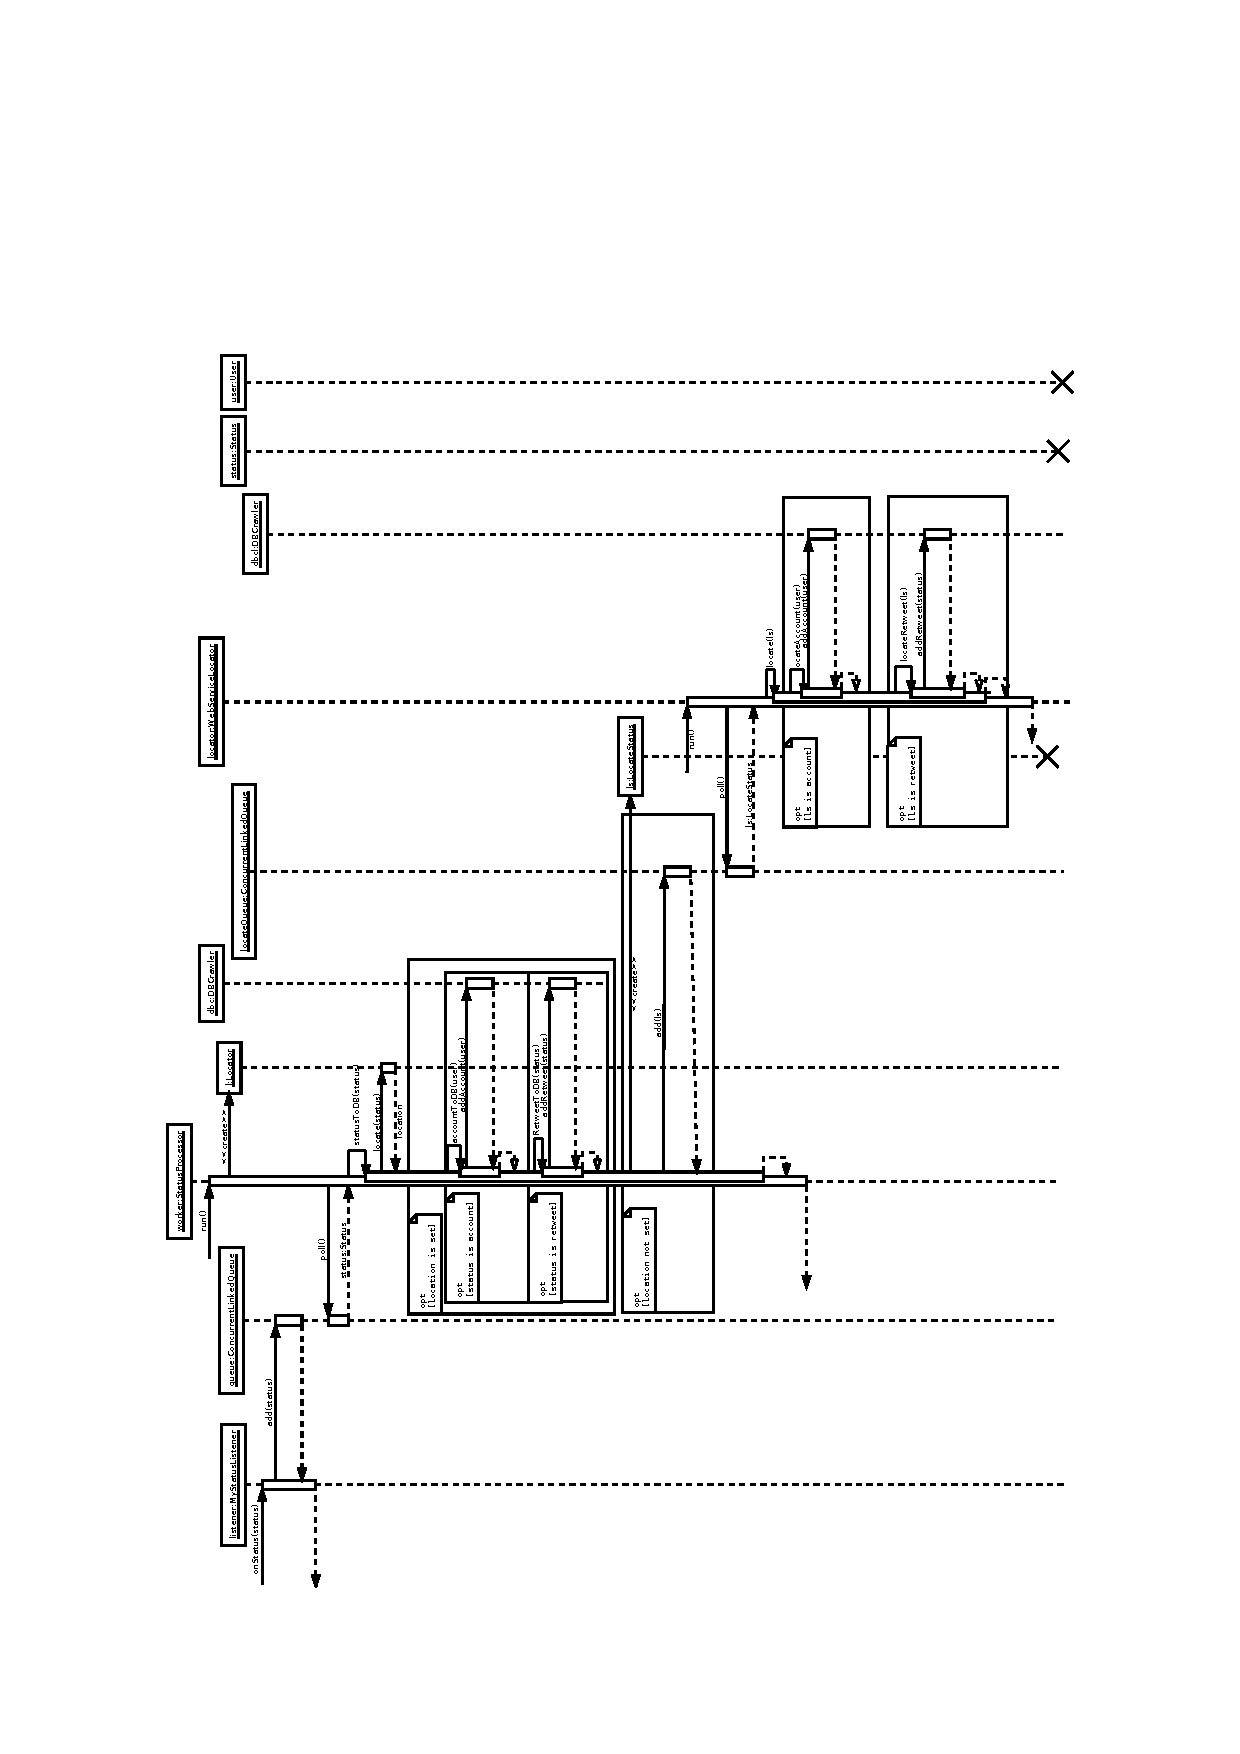
\includegraphics[width=\textheight,height=\textwidth,keepaspectratio=true,angle=-90]{dia/crawler_process_sequence}
	\caption{Sequenzdiagramm der Verarbeitung der Daten von Twitter}
	\label{fig:crawler_process}
\end{figure}

Im Folgenden soll der Weg der Daten von Twitter in unsere Datenbank mit \cref{fig:crawler_process} beschrieben werden.
Zuerst werden die Daten, welche im MyStatusListener auflaufen in eine (threadsichere) Warteschlange geschoben.
Hat dann ein StatusProcessor freie Kapazitäten so entnimmt er das erste Element der Warteschlange. Dieses Status-Objekt enthält alle relevanten Informationen um zu entscheiden ob das Objekt interessant ist oder nicht.
Interessante Status-Objekte enthalten verifizierte Twitter-Accounts oder Retweets auf Tweets von verifizierten Accounts. Ist ein verifizierter Account in einem Status-Objekt gefunden worden, so wird der Account (hier: user) dem Locator zur Lokalisierung übergeben. Dieser versucht dann anhand eines Orts-Strings den Account einem Land zuzuordnen. Ist dies geschehen so wird der Account in die Datenbank geschrieben. Genauso wird auch mit den Status-Objekten verfahren die einen Retweet enthalten.
Ist ein solches Status-Objekt verarbeitet, so beginnt der ganze Verarbeitungsprozess wieder von vorne.

	\chapter{Kategorisierer}
	\label{chap:kategorisierer}
		\section{Aufbau}
Der Kategorisierer wird in regelmäßigen Abständen vom Betriebssystem gestartet und verbindet sich mit der Datenbank. Über die Datenbankschnittstelle ließt er die bislang unkategorisierten Twitteraccounts aus der Accountstabelle aus und sucht in der DMOZ-Datenbank nach passenden Kategorien. Diese werden dann in die Kreuztabelle AccountCategory eingetragen.

Im Diagramm \ref{fig:categorizer} ist der grundlegende Aufbau des Kategorisierers dargestellt:
\begin{figure}[h!]
	\centering
	\includegraphics[width=\textwidth,height=\textheight, keepaspectratio=true]{dia/categorizer}
	\caption{Klassendiagramm des Kategorisierers}
	\label{fig:categorizer}
\end{figure}
\begin{description}
	\item[Account] siehe \cref{sec:datenbankzugriff}
	\item[Category] siehe \cref{sec:datenbankzugriff}
	\item[DBIcategorizer] Über dieses Interface kommuniziert der Kategorsierer mit der Datenbank. Es enthält Methoden zum Holen der unkategorisierten Accounts, zum Finden von Kategorien, zum Eintragen einer Kategorie und zum Auffinden aller Subkategorien einer Kategorie.
	\item[Categorizer] Dies ist die Haupt-Klasse des Kategorisierers. Sie nutzt die Methoden von \lstinline{DBIcategorizer}, um unkategorisierte Accounts zu suchen und gefundene Kategorien einzutragen.
\end{description}

\section{Start des Kategorisierers}
Der Kategorisierer soll in regelmäßigen Abständen vom Betriebssystem gestartet werden und daraufhin die neu gefundenen Accounts kategorisieren.

Der Ablauf des Kategorsierers ist im Sequenzdiagramm \ref{fig:categorizerSeq} zu sehen.
\begin{figure}[h!]
	\centering
	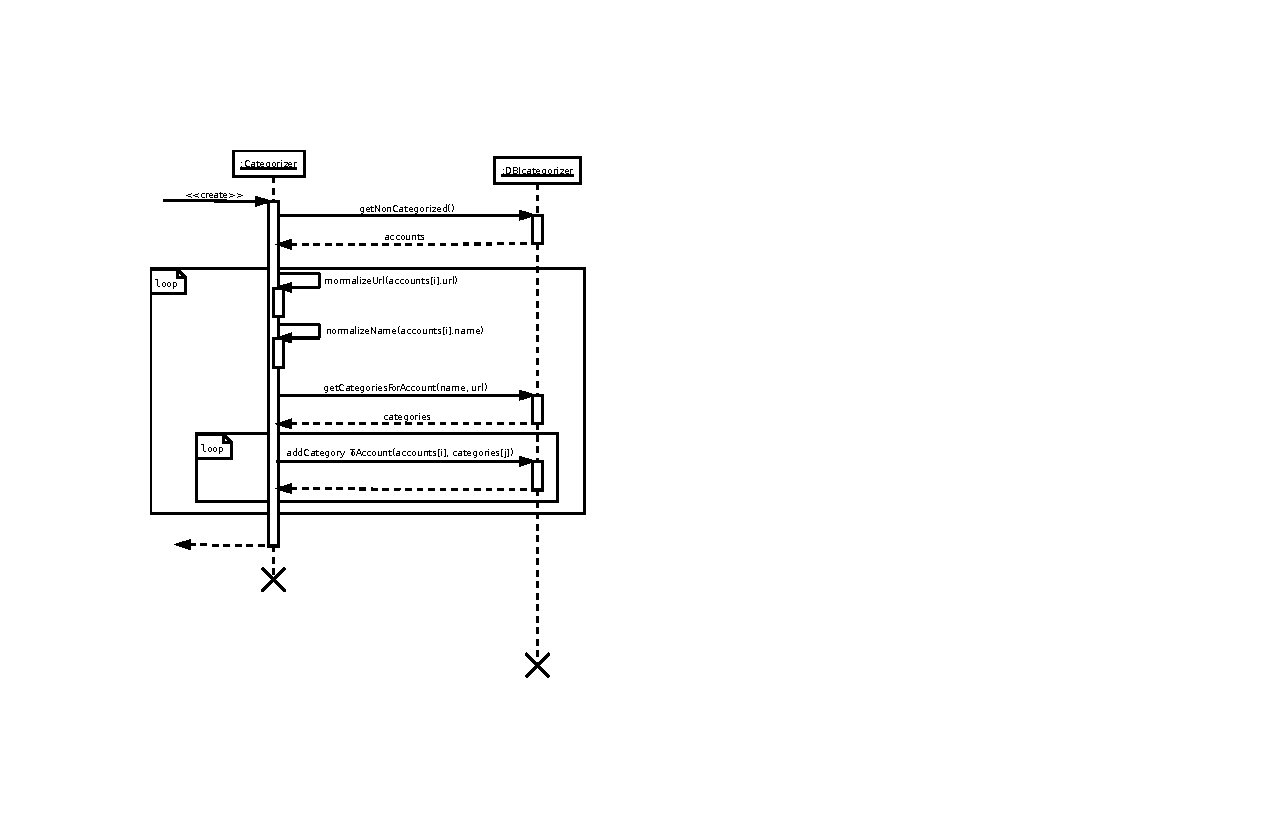
\includegraphics[width=\textwidth,height=\textheight,keepaspectratio=true]{dia/categorizerSequence}
	\caption{Sequenzdiagramm für einen Durchlauf des Kategorisierers. Dabei sind exemplarisch nur jeweils der erste unkategorisierte Account und die erste gefundene Kategorie aufgeführt.}
	\label{fig:categorizerSeq}
\end{figure}

Im ersten Schritt wird also eine Liste von unkategorisierten Accounts ausgelesen. Für jeden dieser Acounts wird eine Liste passender Kategorien ermittelt, die dann nach und nach in die Datenbank geschrieben werden.

	\chapter{GUI}
	\label{chap:gui}
		\section{Aufbau}
\subsection{Paketdiagramm}
\subsection{Klassendiagramm}
Die GUI ermöglicht die Interaktion des Benutzers mit der Anwendung und stellt die über den Crawler gesammelten Daten grafisch aufbereitet dar. 
\begin{figure}[h!]
	\centering
	\includegraphics[width=\textwidth,height=\textheight,keepaspectratio=true]{dia/TwitterGUI_Erweiterung}
	%\includegraphics[width=\textheight,height=\textwidth,keepaspectratio=true,angle=-90]{dia/TwitterGUI_Erweiterung}
	\caption{Klassendiagramm der GUI}
	\label{fig:GUI}
\end{figure}
\begin{description}
	\item[GuiController] Diese Klasse enthält alle GUI-Elemente. Damit kann über diese Klasse jedes einzelne Element angesprochen und damit gesteuert werden. Außerdem speichert sie die jeweils aktuellen Resultate der Datenbankabfragen zentral. Jede Erweiterung muss sich im GuiController als 'Observer' eintragen, um über Änderungen der Daten informiert zu werden. 
	\item[GuiElement] Interface, das jedes GUI-Element implementieren muss.
	\item [selectionOfQuery] Dieses Paket enthält Darstellung und Anwendungslogik für die Auswahl einer Suchanfrage (Auswahl von Kategorie, Land, usw.)
	\item[databaseOptions] Dieses Paket enthält die Darstellung und Anwendungslogik für Änderungen an der Datenbank, wie das Hinzufügen eines bisher nicht mitgetrackten Accounts.
	
	\item [standardMap] Das Paket enthält Anwendungslogik und Darstellung für die Standardkarte, welche die Länder nach dem jeweiligen Tweet-Retweet-Aufkommen einfärbt.
	\item [table] Paket, welches Anwendungslogik und Darstellung für die Erstellungen und Anzeige des Datenblattes zur aktuellen Anfrage enthält.
	\item [timeSliderMap] Paket, welches Anwendungslogik und Darstellung für Erstellung und Anzeige des Tweet-Retweet-Aufkommens in Abhängigkeit des gewählten Zeitraums anzeigt.
	\item [myUnfoldingMap] Diese Klasse kapselt die eigentliche Darstellung sämtlicher Kartenanzeigen. Sie ist die 'Schnittstelle' zur Unfolding-Library, welche für die Anzeige der Weltkarte verwendet wird.
\end{description}
\section{Sequenzdiagramme}
\subsection{GUI Initialisierung}
\begin{figure}[h!]
	\centering
	\includegraphics[width=\textwidth,height=0.5\textheight,keepaspectratio=true]{dia/GUISequenz_Start}
	\caption{Sequenzdiagramm der Initialisierung der GUI.}
	\label{fig:GUIStartSeq}
\end{figure}
\subsection{Kommunikation: GUI und Datenbank}
In \cref{fig:GUISeq} ist die Auswahl einer neuen Kategorie in einem Sequenzdiagramm dargestellt. Der Benutzer klickt auf eine Kategorie in der Liste, woraufhin \emph{handle(mouseEvent)} ausgelöst wird. Der \emph{SelectionOfQuerryController} gibt dieses Ereignis dem \emph{GuiController} weiter bzw. übergibt ihm eine Liste aller IDs ausgewählter Kategorien. Diese Klasse wiederum läd mittels \emph{getData} neue Daten zu den sich geänderten Kategorien. Die IDs ausgewählter Kategorien, Locations und Accounts (siehe Parameter der Operation \emph{getData}) sind dabei lokal in der Klasse \emph{GUIController} gespeichert.

Alle GUI-Elemente werden dann mittels \emph{update} über geänderte Daten informiert. Als Parameter wird ein Enum übergeben, der den Typ der Datenänderung angibt. Es gibt folgende Typen:
\begin{description}
	\item[TWEET] Die Information Anzahl Retweets pro Land und Tweet hat sich geändert. Hier ist bspw. eine Karte, die die Anzahl der Retweets pro Land graphisch darstellt, oder eine Tabelle mit vorher genannten Daten betroffen. 
	\item[CATEGORY] Eine lokale Liste der Kategorien wurde verändert. Die Liste, aus der der Benutzer Kategorien auswählt muss aktualisiert werden.
	\item[LOCATION] Länder bzw. Orte wurden aktualisiert. Auch hier ist z.B. die Liste im Filter, aus dem der Benutzer ein Land auswählt betroffen.
\end{description}
Bei Änderungen vom Typ \emph{TWEET} ist bspw. die \emph{StandardMapView} betroffen und fordert mittels \emph{getTweets()} die neue Informationen an und aktualisiert somit die aktuell angezeigte Karte. Einfachheitshalber wird hier nur die Aktualisierung eines GUI Elements visualisiert. Die Operation \emph{udpate} wird auf jedem GUI-Element, welches sich beim \emph{GUIController} mittels \emph{subscribe} angemeldet hat, aufgerufen.
\begin{figure}[h!]
	\centering
	\includegraphics[width=\textwidth,height=\textheight,keepaspectratio=true]{dia/TwitterGUI_Erweiterung_SequenzDiagramm}
	\caption{Sequenzdiagramm für Auswahl einer neuen Kategorie in der GUI.}
	\label{fig:GUISeq}
\end{figure}

	\chapter{Datenfluss}
	\label{chap:datenfluss}
		\section{Datenflussdiagramm}

Abschließend soll der Datenfluss innerhalb des Programms mithilfe von Abb. 6.1 genauer betrachtet werden.\\

\begin{figure}[h!]
	\centering
	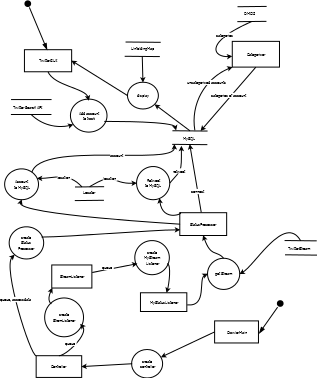
\includegraphics[width=\textwidth,height=0.8\textheight,keepaspectratio=true]{dia/datenflussdiagramm}
	\caption{Datenflussdiagramm des gesamten Systems}
	\label{fig:datenflussdiagramm}
\end{figure}

Der Datenfluss beginnt in der Klasse CrawlerMain, in der die main-Methode gestartet wird. Zuerst fließen dort Zugangsdaten der Datenbank an ein Controller Objekt, welche für seine Erzeugung notwendig sind. \\
Ist dies abgeschlossen werden mehrere StatusProssesor Objekte erzeugt denen jeweils die Queue, in der später die zu verarbeitenden Tweets enthalten sein werden, und Zugangsdaten für die Datenbank übergeben. Diese StatusProcessor Objekte verbinden sich anschließend mit Hilfe der zuvor erhaltenen Zugangsdaten mit der Datenbank. Zeitgleich wird ein StreamListener Objekt erzeugt dem wiederum die vorhin beschriebene Queue und ein Logger Objekt übergeben wird. Sobald diese Initialisierung abgeschlossen ist erzeugt das StreamListener-Objekt ein MyStreamListener, dem es wieder die Queue und einen Logger mitliefert. Sobald dies geschehen ist beginnt der MyStreamListener Daten aus dem TwitterStream auszulesen und sie in die Queue zu schreiben, die der StatusProcessor permanent bearbeitet. Solche Tweet-Objekte fließen also durch die Queue zu einer der StatusProcessor Instanzen. \\
Sobald ein StatusProcessor Objekt erkennt, dass der gerade in Bearbeitung befindlicheTweet von einem verifizierten Account kommt, wird der Account mit Hilfe der Daten, die der Kategorisierer liefert, (dieser benutzt dafür Daten aus der DMOZ-Datenbank) und der Daten, die der Lokalisierer liefert (dieser benutzt den Web-Lokalisierungsdienst), in die Datenbank geladen. Stellt der StatusProcessor fest, dass es ein Retweet war, wird er zusammen mit den Daten aus dem Lokalisierer in die Datenbank geladen.\\
Sind Daten in der Datenbank vorhanden können diese dann auf der TwitterGUI visualisiert werden. Dazu fließen die entsprechenden aufgearbeiteten Daten zusammen mit den notwendigen Daten die für die UnfoldingMap-Darstellung zur GUI. Werden nun in der GUI zusätzlilche Accounts zum Tracken angegeben, werden diese an die Datenbank gesendet und der Kreislauf wird geschlossen.\\
Die TwitterGUI ist somit ein zweiter Startpunkt für den Datenfluss.	
	%end{description}
	\chapter{Glossar}
		% Esentielle Begriffe.

\begin{description}

\end{description}

	\chapter{Größere UML Diagramme}
		% Detaillierte Beschreibung bestimmter für das Programm wichtige Abläufe anhand von Sequenzdiagrammen. Es sollten etwa 3-4 charakteristische und interessante Abläufe ausgewählt werden.

	\listoffigures
\end{document}
